\subsection{Architettura di Progetto e Stack Tecnologico utilizzato}
Per lo sviluppo del nostro progetto abbiamo implementato un'architettura client-server con comunicazione RESTful. La soluzione è strutturata nei seguenti componenti:

\subsubsection*{Frontend}
    \begin{itemize}
    \item Vue.js 3, framework JavaScript progressivo per la costruzione di interfacce utente moderne e reattive
    \end{itemize}
    
\subsubsection*{Backend}
    \begin{itemize}
    \item Node.js, ambiente di runtime JavaScript lato server
    \item Express, framework web minimale e flessibile per la gestione delle richieste HTTP e la definizione delle API
    \item MongoDB, database NoSQL orientato ai documenti per la persistenza dei dati
    \item Firebase Authentication per la gestione delle registrazioni e degli accessi
    \item Jest per l'implementazione dei test delle API
    \end{itemize}
    
\subsubsection*{Strumenti di sviluppo}
    \begin{itemize}
    \item Axios per gestire le chiamate HTTP tra client e server
    \item MongoDB Compass per la visualizzazione e manipolazione diretta dei dati
    \item GitHub per il controllo di versione e la collaborazione nel team
    \item Postman per il test delle chiamate API, in più rispetto a Jest
    \item Visual Studio Code come ambiente di sviluppo integrato
    \end{itemize}

\subsection{Diagramma del deploy finale}

\begin{figure}[h!]
    \centering
    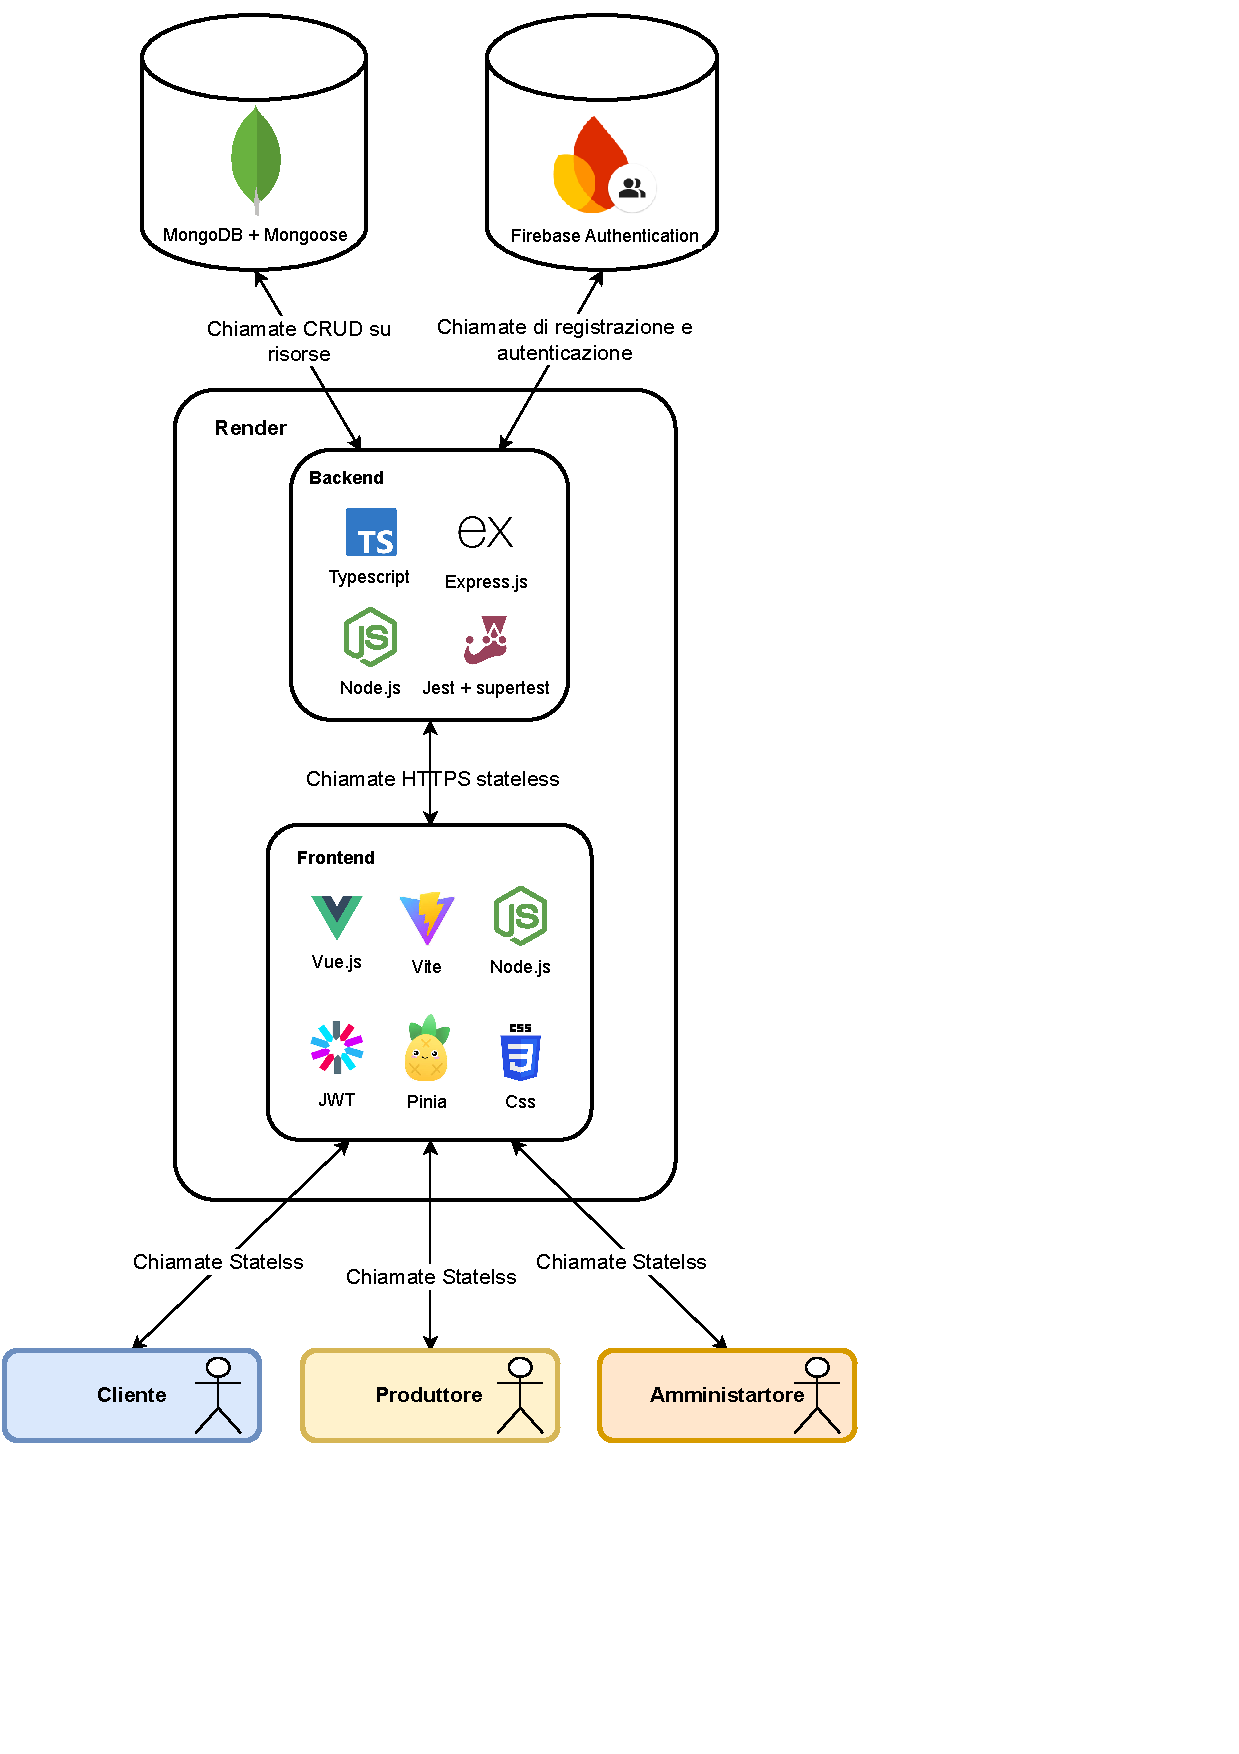
\includegraphics[trim= 0cm 5cm 6.5cm 0cm, clip, width=0.8\linewidth]{Deliverables/fourth-deliverable/img/DiagrammaAgriTrento.drawio.pdf}
    \caption{Deploy finale di AgriTrento}
\end{figure}

\newpage
\subsection{Conclusioni}

Con questo progetto abbiamo imparato davvero molte cose, dall'utilizzare GitHub in un ambiente collaborativo di Team al capire come funziona \verb|Node.js| con il suo Packet manager \verb|npm| fino al Deployment su una piattaforma apposita quale Render.


Sarebbe stato interessante affrontare anche il tema del deploy di container su servizi di orchestrazione quali Google Cloud o altri, ma visto il poco tempo a disposizione sarebbe diventato un ulteriore livello di complicazione considerando che il corso ha durata di soli 6 mesi.

\vspace{0.5cm}

Inoltre, abbiamo acquisito una comprensione approfondita di cosa significhi lavorare in un team composto da più persone: saper conciliare gli impegni e le esigenze di tutti i membri, distribuire efficacemente i compiti e utilizzare framework di sviluppo come l'approccio Agile.
Tuttavia, abbiamo anche notato come quest'ultimo possa talvolta risultare impegnativo, specialmente a causa della documentazione accessoria richiesta dal corso, che rallenta la produttività complessiva del team.

\vspace{0.5cm}

Questo corso è stato, a nostro avviso, il più bello di tutta la triennale che lascia, senza ombra di dubbio, molto a livello pratico.

Nonostante questo però è stato davvero impegnativo soprattutto per l'ultimo sprint dove c'è stato richiesto di creare molte cose accessorie, non valutate a livello accademico, quali: il video per il comune e piano economico per i prossimi anni.
Anche lo stesso deploy per noi è stato un po' complicato essendo che l'ambiente Render, anche se visto a lezione, ci ha dato filo da torcere essendo che ogni applicazione è diversa dalle altre.




